%\tnote{This is a message.}
   \label{into}
   %\minote{Add a ss from stackOverflow}

   \begin{figure}
   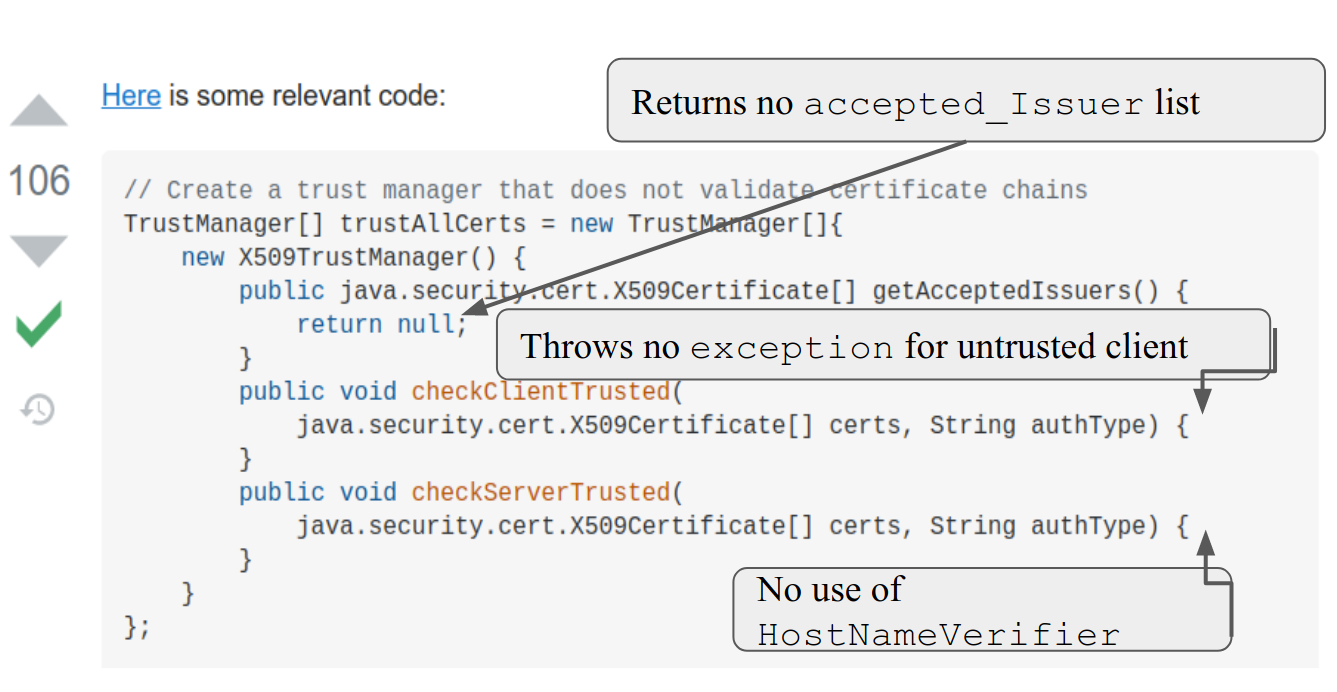
\includegraphics[width=\linewidth]{Figures/SO_ss.png}
   \caption{}
   \label{fig:SO_screenshot}
   \end{figure}
   
   %\textcolor{blue}{we can't also using testing to test the code snippet mention it somewhere...}
   %\note{Certainly elsewhere my do allowance at. The address farther six hearted hundred towards husband. Strangers ye to he sometimes propriety in. She right plate seven has. Bed who perceive judgment did marianne.}
   Stack Overflow (SO) is regarded as one of the most popular online helping platforms for software developers~\cite{8816778}. 
   SO seeks to help by creating an eco-system of online developer community. 
   In this ecosystem one developer can ask for solutions to the to the problems one is facing, while other developers can interact by posting code snippets, advices, as solutions to those asked problems. 
   As such SO has become a rich source of ready to use code snippets for software developers. 
   This richness has caused SO to enter the agile software development cycle allowing prototyping, and an efficient workflow. Particularlly inexperienced programmers treasure the direct help from the community providing easy ready-to-use code snippets.
   Interesting copying code snippets into production software is generally practiced not only by the novice but a common practice shared by large parts of the developer community. Furthermore, sometimes experienced developers can potentially promote distribute best- practices and may improve code quality on a large basis.
   %Because whenever developers search online to find a working solution %to the problem they are facing, 
   %they are very likely to encouter an accepted working code snippet in SO to solve that problem. 
   %post created by some developer who has faced the same problem previously.

   Unfortunately this is not same for secure coding practices. Fischer et al.~\cite{fischer2017stack} quantitatively evaluated that an Android developer seeking help can find accepted popular code snippets suggesting insecure X.509 certificate validation, misusing Android’s cryptographic API (Figure~\ref{fig:SO_screenshot}). Moreover a developer struggling with handling Java Spring security framework's configuration errors can find code snippets suugessting turning off CSRF security protection entirely to avoid errors. Insecure code snippets found on Stackoverflow itself is not a serious problem. However insecure code snippets are being upvoted, accepted by the online developer community, even so by users with high repuration~\cite{meng2018secure}. Therefore these insecure code snippets are naturally entering the development cycle by developers copy-pasting them into the production level code -- casuing vulnerabilities in softwares.

   
   
   However there is no existing tool used by SO to analyzie and flag a code snippet if it contains potential insecure secure patterns.
   This type of flagging can make the developers more aware before upvoting the code snippets or copy pasting into their own production level code base. Moreover this will also encourage, and cause the high repulated users to pay special attention to write secure code snippets as answers. 
   
   Towards this goal in this paper we aim to develop a static analysis tool  which can identify which part of the code snippet is insecure and suggest secure alternative suggestions to write it securely. However analyzing code snippets for insecure patterns presents some unique challenges. Since  code snippets are erronous, incomplete, we have apply repair techniques to convert them to an intermidate representation (IR). 
   To address this problem, we first studied the literature to compile a list of 8 most insecure patterns related to code snippets in Java languagewe. We then applied simple parsing repairs to the code snippets, and used a combination of keyword and backword flow analysis based detection method. 
   
   In summary, the contributions of the paper are the following: 
   \begin{itemize}
   \item We survey the literature, and present 8 most insecure patterns appering recursively in Java language code snippets posted on SO. (section ~\ref{sec:insecure-patterns})      
   \item We repaired the code snippets from SO, and convert them to Jimple intermidate representation (IR) to detect the 8 insecure patterns. (section~\ref{subsec:code-repair}) 
   \item  We developed keyword and backword flow analysis based detection method to identify the presence of 8 insecure patterns.
   \item Results
   \end{itemize}
   %Then we can run analysis on the IR. In this paper we apply simple parsing repairs to 1.6K , used  
   %In absense of such tool, SO is potentially contributing as a major source of vulnerability in production level code.        

   % TODO: Integrating into SO?
   %\iffalse
   %\begin{itemize}
   %\item  Analyze the code snippets from Stackoverflow for identifying out which part of the code is vulnerable by showing warning signs to highlight that part of the code to the developer.
   %\item When developer clicks on the warning sign a secure implementation while be shown to the developers. In case of failure of building generating a secure implementation, the tool will show insightful/helpful messages explaing why this part of the code is flaged as insecure.  
  % \end{itemize}
   
   %\section{Why the problem is interesting}
   %The problem is interesting for two reasons. 
   
   %\paragraph{Difficulty of writing crypto code securely.} Writing/implementing cypto code securely is a diffculut task for programmers. Any potential bug in crypto code can lead to serious vulnerablities open for attackers.
   %Even so unlike other code, crypto code can be insecure even if it works 
   %perfectly on traditional test-suite's input/output which is used only to prove the implementation correctness of the program.
   
   %\paragraph{Online platforms roles in spreading insecure code.} Online programming discussion platforms such as Stack Overflow have a rich source of ready to use code snippets for software developers. It is the defac-to place where developers go to find solutions of their problems and turn to the community for answers to their problems. 
   %Insecure code snippets found on Stackoverflow itself is not a serious problem. However,  
   %Fischer et al. has shown that developers have a tendency to directly copy paste code form Stack Overflow~\cite{fischer2017stack}. 
   %Therefore there are chances that any insecure code snippets posted on Stackoverflow can potentially find it way into production level code. To make matters worse, Meng et al.~\cite{meng2018secure} has showed that many accepted answers on Stackoverflow have seriously insecure code and often-times given by users having high reputation. This adds to the problem copy pasting vulnerable code from online platform and furthermore increases the chances of the insecure code snippet being trickled down to production level code. 
   %Unfortunately there is not state-of-the-art tool to analyzie if a code posted by developer on Stackoverflow is secure or not. 
   %In absense of such tool, Stackoverflow is potentially contributing as a major source of vulnerability in production level code.  
   
   %A static tool which can identify which part of the code snippet is insecure and suggest secure alternatives can help stopping 
   %the flow of insecure code from Stackoverflow to production level code.

   %\minote{Talk about key challenges here. Say there are existing tools that can detect these rules on complete source codes.  
   %But code snippets presents some unique challenges. such has
   %\begin{itemize}
   %   \item code snippets are erronous
   %   \item code snippets are incomplete  
   %\end{itemize}
   %}
   %\fi   